\documentclass[UTF8]{beamer}
\usepackage{ctex}
\usepackage{fontspec}
\usepackage{comment}
\usepackage{xeCJK}
%\setsansfont{Microsoft YaHei}
\setCJKmainfont{Microsoft YaHei}
%\setCJKmonofont{KaiTi}
%\setCJKsansfont{Microsoft YaHei}
\usefonttheme{professionalfonts}
\usepackage{graphicx}
\graphicspath{{fig/}} % storage figure in a sub-folder
% \usepackage[parfill]{parskip} % Activate to begin paragraphs with an empty line rather than an indent
\usepackage{epstopdf}
\usepackage{bm}
\usepackage{pycolor}
\usepackage{pythonhighlight}
\usepackage{hyperref}
\hypersetup{CJKbookmarks=true}
\usepackage{url}
\usepackage{amsmath}
\usepackage{amsthm}
%\theoremstyle{definition}
%\newtheorem{theorem}{定理}
%\newtheorem{definition}{定义}
%\newtheorem{corollary}{推论}
%\newtheorem{example}{例}
\usepackage{booktabs} % for much better looking tables
\usepackage{cite} % reference
\usepackage{array} % for better arrays (eg matrices) in maths
%\usepackage{paralist} % very flexible & customisable lists (eg. enumerate/itemize, etc.)
\usepackage{verbatim} % adds environment for commenting out blocks of text & for better verbatim
\usepackage{subfig} % make it possible to include more than one captioned figure/table in a single float
% These packages are all incorporated in the memoir class to one degree or another...
%\usepackage{threeparttable}
\usepackage{cases} %equation set
\usepackage{multirow} %use table
\usepackage{enumerate}
\usepackage{algorithm}
\usepackage{algorithmic}
\usepackage{xcolor}
%\usepackage{capt-of}
\setcounter{tocdepth}{1}%只显示section,不显示subsection
\usepackage{listings}
\lstset{tabsize=4, keepspaces=true,
    xleftmargin=2em,xrightmargin=0em, aboveskip=1em,
    backgroundcolor=\color{gray!20},  % 定义背景颜色
    frame=none,                       % 表示不要边框
    extendedchars=false,              % 解决代码跨页时,章节标题,页眉等汉字不显示的问题
    numberstyle=\ttfamily,
    basicstyle=\ttfamily,
    keywordstyle=\color{blue}\bfseries,
    breakindent=10pt,
    identifierstyle=,                 % nothing happens
    commentstyle=\color{green}\small,  % 注释的设置
    morecomment=[l][\color{green}]{\#},
    numbers=left,stepnumber=1,numberstyle=\scriptsize,
    showstringspaces=false,
    showspaces=false,
    flexiblecolumns=true,
    breaklines=true, breakautoindent=true,breakindent=4em,
    escapeinside={/*@}{@*/},
}

\title[Beamer模板]{Style of Nankai University}
\subtitle{Beamer模板}
\author[李华]{李华\\(\url{lihua@163.com})}
\institute{南开大学XX学院}
%\author[Calvin]{Calvin\inst{1} \and Cleven\inst{2}}
%\institute[Univ]{\inst{1}南开大学 \and \inst{2}克莱登大学}
\date{\today}


\begin{document}
%%%%%%%%%% 定理类环境的定义 %%%%%%%%%%
%% 必须在导入中文环境之后

\renewcommand{\contentsname}{目录}     % 将Contents改为目录
\renewcommand{\abstractname}{摘要}     % 将Abstract改为摘要
\renewcommand{\refname}{参考文献}      % 将References改为参考文献
\renewcommand{\indexname}{索引}
\renewcommand{\figurename}{图}
\renewcommand{\tablename}{表}
\renewcommand{\appendixname}{附录}
%\renewcommand{\proofname}{证明}
%\renewcommand{\algorithm}{算法}
%----------------------------------------------------------------------
% Title frame
\begin{frame}[plain]
\maketitle
\end{frame}

%----------------------------------------------------------------------
% Outline frame

\begin{frame}
\frametitle{目录}
\tableofcontents
\end{frame}
%%=====================================================================
% Section I
\section{框架}
%----------------------------------------------------------------------
% Content frame

\subsection{测试功能}

\begin{frame}
    \begin{figure}
        \centering
        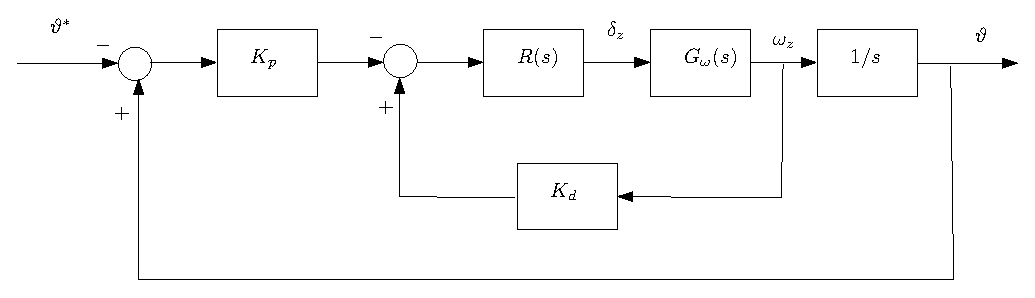
\includegraphics[width=0.9\textwidth]{vart.eps}
    \end{figure}
\end{frame}

\begin{frame}{枚举}
    \begin{enumerate}
        \item No one has done it.
        \item I need one.
    \end{enumerate}
\end{frame}

\begin{frame}{算法}
    \begin{algorithm}[H]
        \caption{背景减除}
        \begin{algorithmic}[1]
            \STATE 初始化
            \REPEAT
            \STATE 获取第t帧图像
            \UNTIL{所有帧都被处理}
        \end{algorithmic}
    \end{algorithm}
\end{frame}

\subsection{basic frame}

\begin{frame}[allowframebreaks]
\frametitle{框架:Why I made this}
%\framesubtitle{Why I made this beamer style}
\begin{block}{Demonstration of the use of items and blocks}
\begin{itemize}
\item No one has done it.$$e=mc^2$$
\item I need one.
\pause \item Share with others.
\end{itemize}
\end{block}
\pause
\begin{block}{Another block}
This block appears after a pause. Simply delete the \texttt{\textbackslash pause} command if this animation is not needed. Add the pause command whenever a pause is needed. 
\end{block}
\end{frame}

%%=====================================================================
% Section II
\section{extend usage}
%----------------------------------------------------------------------
\subsection{format}
\begin{frame}
\frametitle{A Two-column Slide}
\begin{columns} 
\begin{column}{0.5\textwidth} 
\begin{figure}[htb]
	
\includegraphics[width=2.5cm,height=1.3cm]{test.png}
	\caption{插入图片示例}
	\label{fig1}
    \end{figure}
\end{column}
\begin{column}{0.5\textwidth} 
颜色如图\ref{fig1},以及 e.g. {\color{red}{red}}, {\color{orange}{orange}}, {\color{blue}{blue}}
\vspace{9.5em}
\end{column}
\end{columns}
\end{frame}

\begin{frame}
    \frametitle{无序列表}
    \begin{description}
        \item[i] first of all
        \item[ii] besides
        \item[iii] last but not least
    \end{description}
    \begin{equation}
        \text{e}^{\pi \text{j}} + 1 = 0
    \end{equation}
    \begin{itemize}
        \item first
        \item second
    \end{itemize}
\end{frame}

\begin{frame}{表格}
\begin{table}[!hbp]
\centering
\begin{tabular}{c|c}
	\hline
	甲 &乙\\
	\hline
	11 & 12\\
	21 & 22\\
	31 & 32\\
	\hline
\end{tabular}
\caption{插入表格示例}
\label{tab1}
\end{table}
\end{frame}

\begin{frame}[fragile]
    \frametitle{code highlight}
    \begin{lstlisting}[language=java]
public class Hello{
    public static void main(String args[]){
        System.out.println("hello,world");
    }
}\end{lstlisting}
\end{frame}

\begin{python}
import numpy as np
import matplotlib.pyplot as plt
import rec
import math

C = rec.data
print(C)
A = rec.initMat(C)
print(A)
S = rec.svdEst(A)
print(S)

m,n  = A.shape
B = np.dot(S,A.T).T
plt.imshow(B)
x = []
y = []

for i in range(m):
	print(np.sum(S[i,:]))
	for j in range(n):
		if C[i,j] != 0:
			x.append(A[i,j])
			y.append(B[i,j])


plt.scatter(x,y)
#plt.xlim(1,5)
#plt.ylim(0,5)
xt = [1.0,5.0]
plt.title("svd after change")
#print(C)

plt.show()\end{python}

\begin{frame}
    \frametitle{theorem and proof}
    \begin{exampleblock}{Theorem 1 (L\'{e}vy)}
    令 $F(x),\varphi(t)$ 分别为随机变量 $X$ 的分布函数和特征函数。
    假定 $F(x)$ 在 $a+h$ 和 $a-h (h>0)$ 处连续,则有
    \begin{align}
    \label{Levy theorem}  % 方程的标记可以是专有名词
    F(a+h)-F(a-h)&=\lim_{T\rightarrow\infty}\frac{1}{\pi}\int^{T}_{-T}\frac{\sin ht}{t}
    e^{-ita}\varphi(t)dt
    \end{align}
    \end{exampleblock}
    \begin{proof}
        略。
    \end{proof}
    \begin{alertblock}
        Test block!
    \end{alertblock}
\end{frame}

\subsection{总结与致谢}

\begin{frame}
    \frametitle{reference}
    \begin{thebibliography}{99} 
    \bibitem{edwurd} These files are based on Edward Hartley's work
        (\url{http://www-control.eng.cam.ac.uk/Main/EdwardHartley})
    \bibitem{beihang} Beamer style of Beihang
    \end{thebibliography}
\end{frame}

\begin{frame}
    \centering{\Huge{谢谢大家!}}\\
\end{frame}
\end{document}
